% !TEX program = xelatex
% Editable LaTeX source for the 15-minute presentation.
% Compile main.tex with XeLaTeX for the confirmed 15-minute talk.
\RequirePackage{fix-cm}
\documentclass[11pt,aspectratio=169,xcolor={dvipsnames}]{beamer}
\usetheme[progressbar=frametitle,block=fill]{metropolis}
\usefonttheme{professionalfonts}
\usepackage{lmodern}
\usepackage{fontspec}
\setsansfont{texgyreheros}[Extension=.otf,UprightFont=*-regular,BoldFont=*-bold,ItalicFont=*-italic,BoldItalicFont=*-bolditalic]
\usepackage{booktabs,tabularx,graphicx,amsmath,tikz,qrcode}
\usetikzlibrary{arrows.meta,positioning,calc}
% Canonical author and credit strings copied from the checked paper.
\newcommand{\PaperTitle}{Fossil Fuel Prices and Capital Cost: A Machine Learning Driven Study on Energy Transition}
\newcommand{\AuthorNames}{Shilin Ou, Luyao Zhang, and Ming-Chun Huang}
\newcommand{\AuthorNamesMarked}{Shilin Ou\textsuperscript{\dag}, Luyao Zhang\textsuperscript{*}, and Ming-Chun Huang\textsuperscript{*}}
\newcommand{\PaperAffiliation}{Duke Kunshan University, Suzhou, China}
\newcommand{\PresenterName}{Shilin Ou}
\newcommand{\PresenterEmail}{shilin.ou@dukekunshan.edu.cn}
\newcommand{\CorrespondenceText}{Corresponding authors: Zhang: luyao.zhang@dukekunshan.edu.cn, Social Science Division and Digital Innovation Research Center; Huang: mingchun.huang@dukekunshan.edu.cn, Natural and Applied Science Division and Digital Innovation Research Center, Duke Kunshan University. Address: No.8 Duke Ave., Kunshan, Jiangsu 215316, China.}
\newcommand{\FundingText}{The Duke Kunshan University Education Development Foundation supports the research. The research results of this article are also sponsored by the Kunshan Municipal Government research funding.}
\newcommand{\AuthorNoteText}{Shilin benefited from scholarly exchange with participants in the AAAI-26 Workshop on AI for Environmental Science, held on January 27, 2026, at the Singapore EXPO in Singapore. Shilin gratefully acknowledges the Travel Grant provided by the Duke Kunshan University Office of Academic Services, which supported participation in the workshop.}
\newcommand{\PreparationText}{OpenAI Codex assisted language and consistency revisions throughout the manuscript, preparation of Fig. 1, and correction of the sensitivity-analysis code.}
\newcommand{\CodeURL}{https://github.com/GreenComp-ERC/ImpactOfFossilFeulPrice}
\newcommand{\DataURL}{https://huggingface.co/datasets/global-nomad-nexus/ImpactOfFossilFuelPrice-WACC}
\newcommand{\EventName}{2026 Asian Conference on Artificial Intelligence Technology}
\newcommand{\EventShort}{ACAIT 2026}
\newcommand{\EventPlace}{Chongqing, China}

\definecolor{DukeNavyBlue}{HTML}{012169}
\definecolor{DukeRoyalBlue}{HTML}{00539B}
\definecolor{Teal}{HTML}{247F83}
\definecolor{Gold}{HTML}{B3853A}
\definecolor{SoftBlue}{HTML}{EAF3FF}
\definecolor{PaperGray}{HTML}{4E5A66}
\definecolor{ModelBlue}{HTML}{173C5B}
\setbeamercolor{normal text}{fg=black!88,bg=white}
\setbeamercolor{frametitle}{bg=white,fg=DukeNavyBlue}
\setbeamercolor{progress bar}{fg=Teal,bg=black!10}
\setbeamercolor{title separator}{fg=DukeRoyalBlue}
\setbeamercolor{alerted text}{fg=DukeRoyalBlue}
\setbeamercolor{block title}{fg=DukeRoyalBlue,bg=SoftBlue}
\setbeamercolor{block body}{fg=black!88,bg=SoftBlue}
\setbeamertemplate{navigation symbols}{}
\setbeamersize{text margin left=0.65cm,text margin right=0.65cm}
\setbeamertemplate{frame footer}{\textcolor{PaperGray}{\EventShort\quad|\quad\PresenterName}}
\setbeamerfont{frame footer}{size=\tiny}
\setbeamerfont{frametitle}{size=\Large,series=\bfseries}
\setbeamertemplate{frametitle}{\vspace{0.25cm}{\usebeamerfont{frametitle}\insertframetitle\par}\vspace{0.10cm}{\color{DukeRoyalBlue}\rule{\textwidth}{0.7pt}}\vspace{-0.15cm}}
\setbeamerfont{title}{size=\LARGE,series=\bfseries}
\setbeamerfont{subtitle}{size=\small}
\hypersetup{pdftitle={\PaperTitle},pdfauthor={Shilin Ou, Luyao Zhang, Ming-Chun Huang},colorlinks=true,urlcolor=DukeRoyalBlue}
\newcommand{\source}[1]{\par\vfill{\fontsize{6.3}{7.5}\selectfont\color{PaperGray}\raggedright #1\par}}
\newcommand{\lead}[1]{{\large\color{DukeNavyBlue}\bfseries #1}\par\medskip}
\newcommand{\smalllabel}[1]{{\scriptsize\color{PaperGray}#1}}
\graphicspath{{../shared/figures/}}
% Native labels over original artwork. Images and numerical curves are unchanged.
\definecolor{PaperModelBlue}{HTML}{173C5B}
\definecolor{PaperXGB}{HTML}{800080}
\newcommand{\PaperNetwork}[2]{%
\resizebox{#1}{!}{\begin{tikzpicture}
\node[anchor=south west,inner sep=0] at (0,0) {\includegraphics[height=5.10cm]{#2}};
\node[fill=PaperModelBlue,text=white,minimum width=0.78cm,minimum height=0.20cm,inner sep=0pt,font=\fontsize{6.2}{7}\selectfont] at (2.11,4.42) {GPR};
\end{tikzpicture}}}
\newcommand{\PaperOilComparison}[2]{%
\resizebox{#1}{!}{\begin{tikzpicture}
\node[anchor=south west,inner sep=0] at (0,0) {\includegraphics[width=12.5cm]{#2}};
\fill[white] (10.97,4.06) rectangle (12.25,5.27);
\draw[black!15,line width=0.4pt] (10.97,4.06) rectangle (12.25,5.27);
\draw[blue,line width=0.7pt] (11.05,5.12)--(11.24,5.12);
\fill[blue] (11.145,5.12) circle (0.018);
\draw[green!45!black,line width=0.9pt] (11.05,4.90)--(11.24,4.90);
\draw[red,dash dot,line width=0.7pt] (11.05,4.68)--(11.24,4.68);
\draw[PaperXGB,densely dotted,line width=0.8pt] (11.05,4.46)--(11.24,4.46);
\draw[orange,line width=0.7pt] (11.05,4.24)--(11.24,4.24);
\foreach \y/\lab in {5.12/Actual,4.90/LSTM-GPR,4.68/SARIMA,4.46/XGBoost,4.24/LightGBM}{
\node[anchor=west,inner sep=0,font=\fontsize{4.7}{5.2}\selectfont] at (11.31,\y) {\lab};}
\end{tikzpicture}}}
\newcommand{\PaperMethodology}[2]{%
\resizebox{#1}{!}{\begin{tikzpicture}[x=1bp,y=1bp]
\node[anchor=south west,inner sep=0] at (0,0) {\includegraphics[width=1313.03992bp]{#2}};
% Correct the summation dummy variable to match the manuscript loss function.
\fill[white] (207,176) rectangle (402,273);
\node[align=center,inner sep=0,font=\fontsize{15}{20}\selectfont] at (304,227) {$\widehat\Theta_h=\arg\min_{\Theta_h}\mathcal L_h$\\[3bp]$\displaystyle\mathcal L_h=\frac{1}{T-h}\sum_{t=1}^{T-h}\varepsilon_t^2$\\[3bp]$\varepsilon_t=y_{t+h}-G(x_t;\Theta_h)$};
\end{tikzpicture}}}


\begin{document}

\begin{frame}[plain]
\begin{tikzpicture}[remember picture,overlay]
\node[anchor=north west,inner sep=0] at ([xshift=0.70cm,yshift=-0.45cm]current page.north west) {
\includegraphics[height=0.72cm]{acait_logo.png}};
\node[anchor=north east,inner sep=0] at ([xshift=-0.70cm,yshift=-0.42cm]current page.north east) {
\includegraphics[width=3.3cm]{dku_logo.png}};
\draw[DukeRoyalBlue,line width=0.7pt] ([xshift=0.70cm,yshift=-1.55cm]current page.north west)--([xshift=-0.70cm,yshift=-1.55cm]current page.north east);
\node[anchor=north west,text width=14.2cm,inner sep=0,text=DukeNavyBlue] at ([xshift=0.70cm,yshift=-2.0cm]current page.north west) {\fontsize{29}{34}\selectfont\bfseries Fossil Fuel Prices\\and Capital Cost};
\node[anchor=north west,text width=13.8cm,inner sep=0] at ([xshift=0.74cm,yshift=-4.65cm]current page.north west) {\fontsize{16}{21}\selectfont A Machine Learning Driven Study on Energy Transition};
\node[anchor=north west,text width=14.2cm,inner sep=0] at ([xshift=0.74cm,yshift=-6.10cm]current page.north west) {\small\AuthorNamesMarked\\[0.20cm]\PaperAffiliation};
\node[anchor=south west,text width=14.2cm,inner sep=0,text=PaperGray] at ([xshift=0.74cm,yshift=0.55cm]current page.south west) {\scriptsize\EventShort\quad\EventPlace\hfill Presented by \PresenterName};
\end{tikzpicture}
\note{\CorrespondenceText\par\FundingText\par\AuthorNoteText\par\PreparationText}
\end{frame}

\begin{frame}{Research question}
\lead{How do fossil fuel prices relate to energy-project financing costs?}
\begin{columns}[T,onlytextwidth]
\column{0.55\textwidth}
\begin{itemize}
\item Debt and equity providers require a return on the capital they commit.
\item A higher financing cost raises the revenue a project must earn.
\item Regional financing differences can change modeled transition pathways.
\end{itemize}
\column{0.40\textwidth}
\vspace{0.35cm}
{\color{DukeRoyalBlue}\Large WACC}\\[0.3cm]
\small Weighted average cost of capital
\[
\underbrace{Lr_D(1-\tau)}_{\text{debt}}+
\underbrace{(1-L)r_E}_{\text{equity}}
\]
\end{columns}
\source{Ameli et al., Nature Communications (2021); Calcaterra et al., Nature Energy (2024).}
\end{frame}

\begin{frame}{Price transmission channels}
\lead{What links fossil fuel prices to energy-project WACC?}
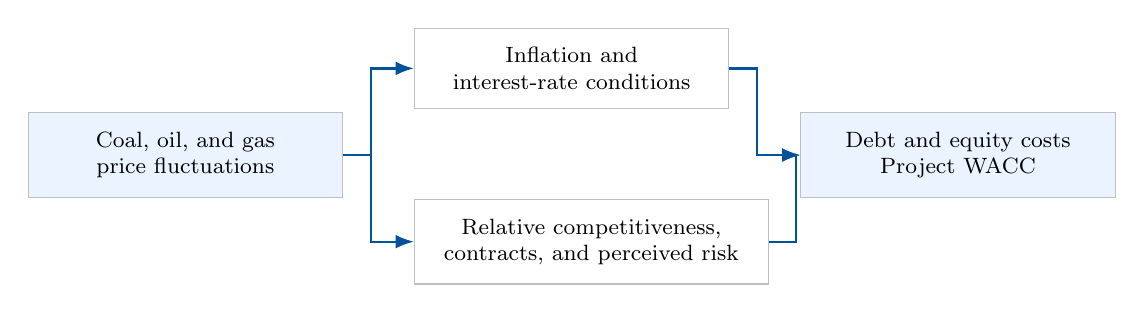
\begin{tikzpicture}[>=Latex,font=\footnotesize,
 b/.style={align=center,text width=3.5cm,minimum height=1.0cm,draw=black!25,fill=white,inner sep=7pt},
 a/.style={->,thick,draw=DukeRoyalBlue}]
\node[b,fill=SoftBlue] (fuel) {Coal, oil, and gas\\price fluctuations};
\node[b,right=0.9cm of fuel,yshift=1.10cm] (macro) {Inflation and\\interest-rate conditions};
\node[b,right=0.9cm of fuel,yshift=-1.10cm,text width=4.0cm] (project) {Relative competitiveness,\\contracts, and perceived risk};
\node[b,right=0.9cm of macro,yshift=-1.10cm,fill=SoftBlue] (wacc) {Debt and equity costs\\Project WACC};
\draw[a] (fuel.east)--++(0.35,0)|-(macro.west);
\draw[a] (fuel.east)--++(0.35,0)|-(project.west);
\draw[a] (macro.east)--++(0.35,0)|-(wacc.west);
\draw[a] (project.east)--++(0.35,0)|-(wacc.west);
\end{tikzpicture}
\par
\medskip
\small We compare these signals across China, Europe, and the Middle East.
\source{Mechanisms from Melodia and Karlsson (2022), Lieberman and Doherty (2007), and Duma and Muñoz Cabré (2023).}
\end{frame}

\begin{frame}{Data and scope}
\begin{tabularx}{\linewidth}{@{}p{0.20\linewidth}X p{0.24\linewidth}@{}}
\toprule
\textbf{Input} & \textbf{Content} & \textbf{Role}\\
\midrule
Fuel prices & Monthly coal, oil, and natural gas series & Price-forecast inputs\\[0.2cm]
Macroeconomy & Inflation, growth, unemployment, interest-rate and monetary indicators & Regional inflation forecasts\\[0.2cm]
WACC & Calcaterra et al. model projections, aligned to 2026--2035 & Financing scenarios\\
\bottomrule
\end{tabularx}
\vspace{0.25cm}
\begin{columns}[T,onlytextwidth]
\column{0.46\linewidth}
\textbf{3 regions}\quad China, Europe, Middle East\\
\textbf{120 monthly rows}\quad per cleaned region
\column{0.50\linewidth}
\textbf{9 technologies}\quad wind, solar, hydro, biomass, nuclear, CCS, coal, and gas
\end{columns}
\source{WACC scenario data: Calcaterra et al. (2024). Coal and gas generation provide conventional-technology comparisons.}
\end{frame}

\begin{frame}{Three-stage framework}
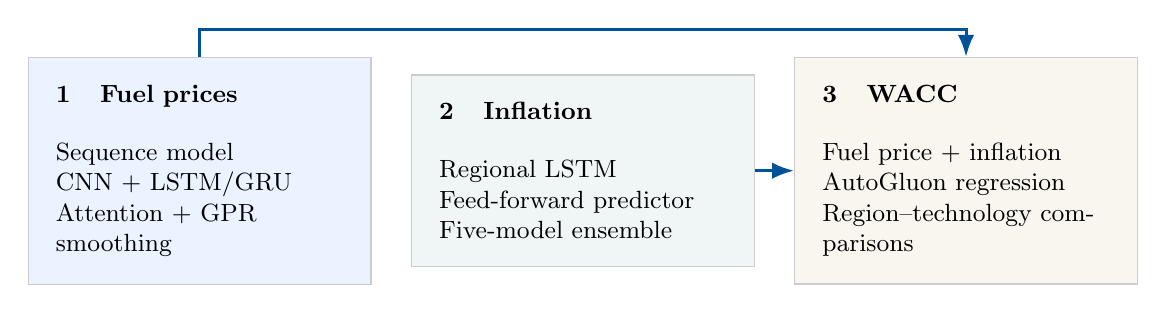
\begin{tikzpicture}[>=Latex,font=\small,
 b/.style={align=left,text width=3.65cm,minimum height=2.2cm,inner sep=10pt,draw=black!20},
 a/.style={->,line width=1.1pt,draw=DukeRoyalBlue}]
\node[b,fill=SoftBlue] (p) {\textbf{1\quad Fuel prices}\\[0.35cm]Sequence model\\CNN + LSTM/GRU\\Attention + GPR smoothing};
\node[b,right=0.5cm of p,fill=Teal!7] (i) {\textbf{2\quad Inflation}\\[0.35cm]Regional LSTM\\Feed-forward predictor\\Five-model ensemble};
\node[b,right=0.5cm of i,fill=Gold!8] (w) {\textbf{3\quad WACC}\\[0.35cm]Fuel price + inflation\\AutoGluon regression\\Region--technology comparisons};
\draw[a] (p.north)--++(0,0.35)-|(w.north);\draw[a] (i)--(w);
\end{tikzpicture}\par
\vspace{0.55cm}
\textbf{Comparison structure}\quad 3 regions $\times$ 3 fuels $\times$ 9 technologies = 81 combinations
\source{Paper Figs. 1--2.}
\end{frame}

\begin{frame}[t]{Fuel-price forecasting model}
\vspace{0.16cm}
\begin{columns}[T,onlytextwidth]
\column{0.40\textwidth}\centering\vspace{0pt}
\PaperNetwork{4.273cm}{paper_LSTM.png}
\column{0.55\textwidth}\vspace{0pt}
\lead{Temporal learning and GPR smoothing}
\begin{itemize}
\setlength\itemsep{0.18cm}
\item A 12-month input window
\item CNN, recurrent layers, and attention
\item Seasonal and rolling-price features
\item Gaussian-process smoothing
\end{itemize}
\vspace{0.3cm}
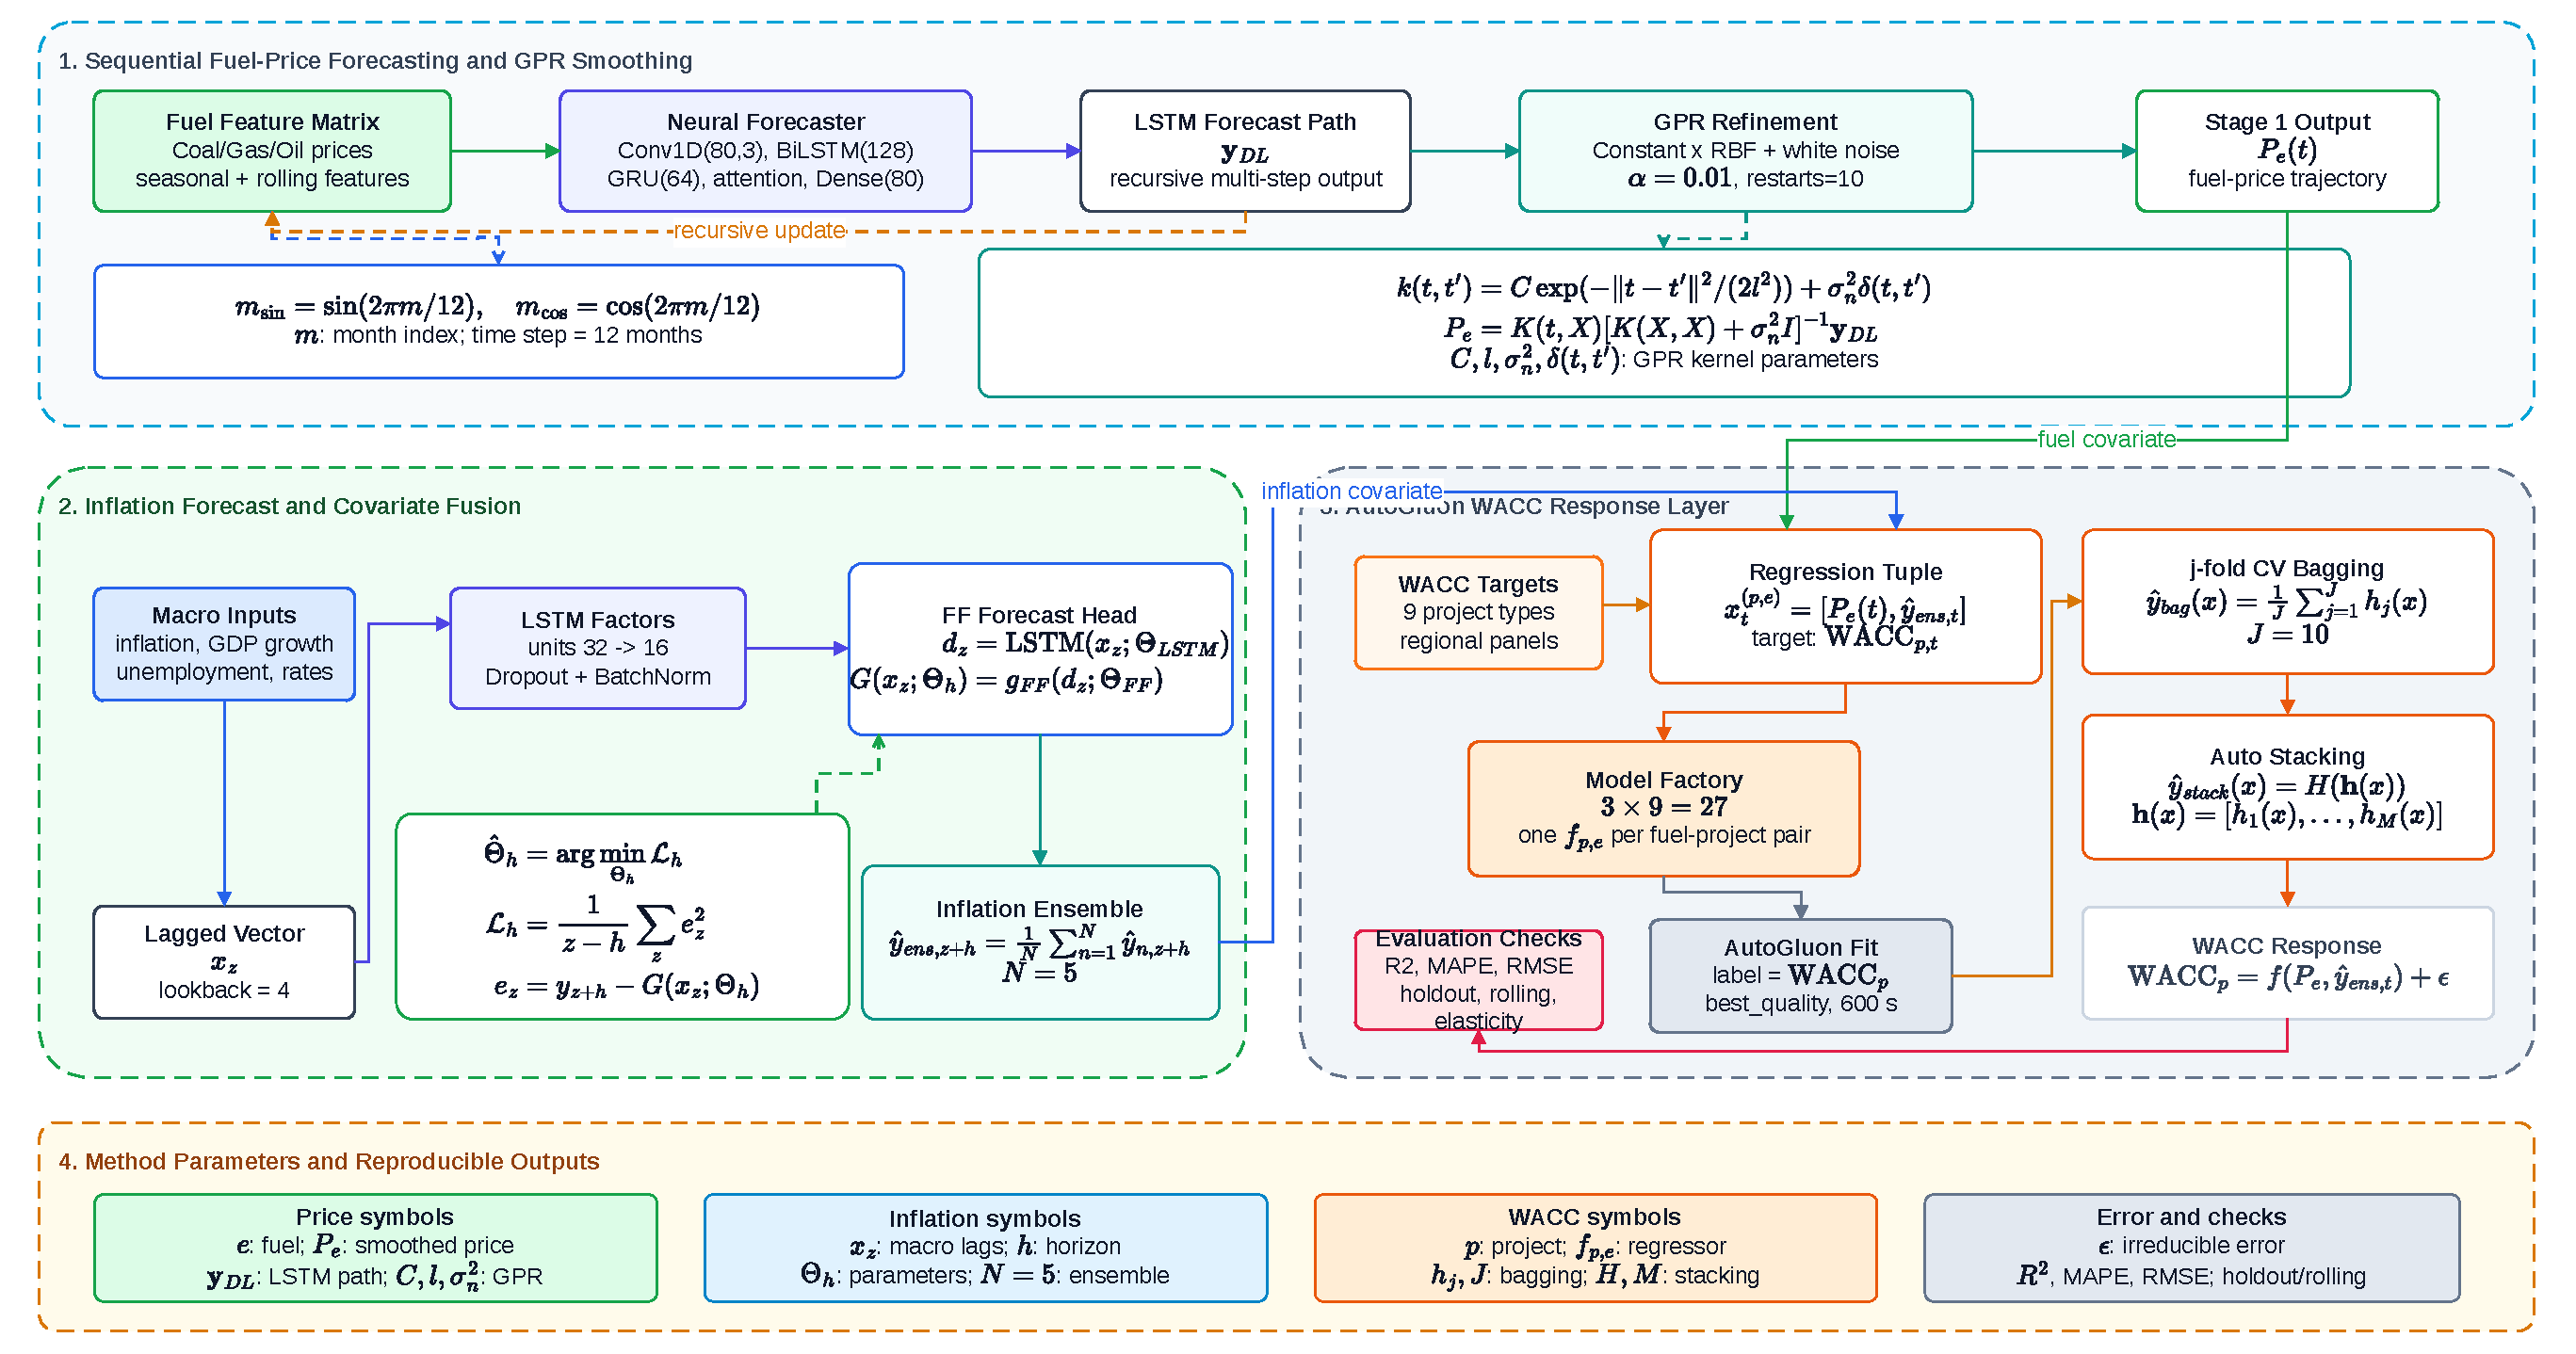
\includegraphics[width=\linewidth,trim=0 470 0 0,clip]{paper_methodology.pdf}
\end{columns}
\source{Paper Figs. 2--3.}
\end{frame}

\begin{frame}{Oil-price comparison, 2021--2024}
\begin{columns}[c,onlytextwidth]
\column{0.75\textwidth}\centering
\PaperOilComparison{\linewidth}{paper_Accuracy.png}
\column{0.21\textwidth}
{\Large\color{DukeRoyalBlue}0.963}\\[-0.05cm]\small $R^2$\\[0.45cm]
{\Large\color{DukeRoyalBlue}1.86\%}\\[-0.05cm]\small MAPE\\[0.45cm]
{\Large\color{DukeRoyalBlue}2.416}\\[-0.05cm]\small RMSE (USD/bbl)
\end{columns}
\source{Paper Fig. 4; metrics recomputed from the 47 saved monthly observations.}
\end{frame}

\begin{frame}{WACC estimation and validation}
\begin{columns}[T,onlytextwidth]
\column{0.47\textwidth}
\lead{AutoGluon regression}
\[
\mathrm{WACC}_{r,p,t}=f_{r,p,e}(P_{e,t},\pi_{r,t})
\]
\begin{itemize}
\item One fuel price and an inflation covariate
\item Bagging and stacking
\item In-sample $R^2$, MAPE, and RMSE
\end{itemize}
\column{0.48\textwidth}
\lead{Time-split validation}
\begin{itemize}
\item OLS/Ridge with cleaned regional inputs
\item Train 2026--2032; test 2033--2035
\item Rolling one-year-ahead checks
\item Compare fuel + inflation + trend against a time trend
\end{itemize}
\end{columns}
\source{Original AutoGluon fit and cleaned-input OLS/Ridge validation are reported separately.}
\end{frame}

\begin{frame}{Regional results}
\begin{columns}[c,onlytextwidth]
\column{0.64\textwidth}
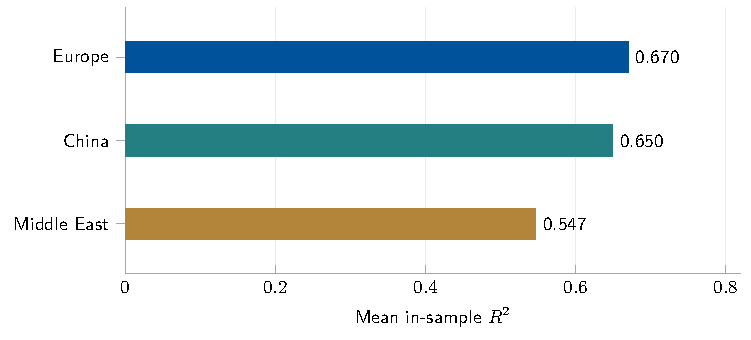
\includegraphics[width=\linewidth]{region_fit.pdf}
\column{0.32\textwidth}
\lead{Europe and China show stronger fit.}
\small Middle Eastern specifications have a lower average fit and larger percentage errors.
\par\vspace{0.25cm}
{\scriptsize\color{PaperGray}Mean $R^2$ across the 27 fuel--technology specifications per region.\par}
\end{columns}
\source{Paper Fig. 5 and results workbook; joint fuel-price and inflation inputs. $R^2$ measures in-sample model fit.}
\end{frame}

\begin{frame}{Technology results}
\centering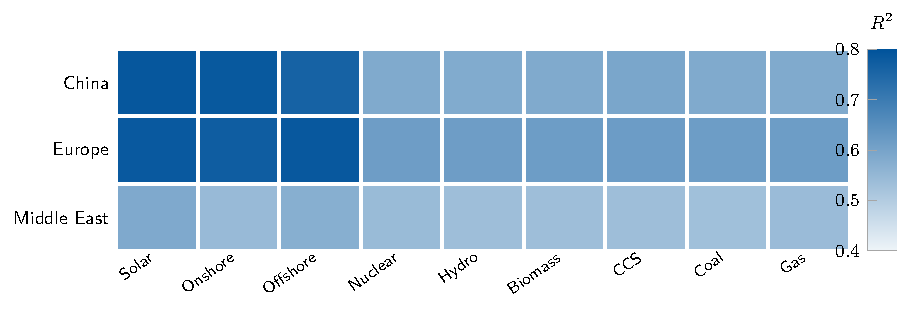
\includegraphics[width=0.88\linewidth]{technology_fit.pdf}\par
\smallskip
\begin{columns}[T,onlytextwidth]
\column{0.53\textwidth}
\textbf{Solar}\quad 0.718\qquad\textbf{Offshore wind}\quad 0.706
\column{0.43\textwidth}
\textbf{Onshore wind}\quad 0.700
\end{columns}
\source{Technology means across three fuels and three regions; heatmap cells average across fuels. Nuclear, hydro, biomass, CCS, coal, and gas are around 0.58 overall.}
\end{frame}

\begin{frame}{Validation over time}
\begin{columns}[c,onlytextwidth]
\column{0.62\textwidth}
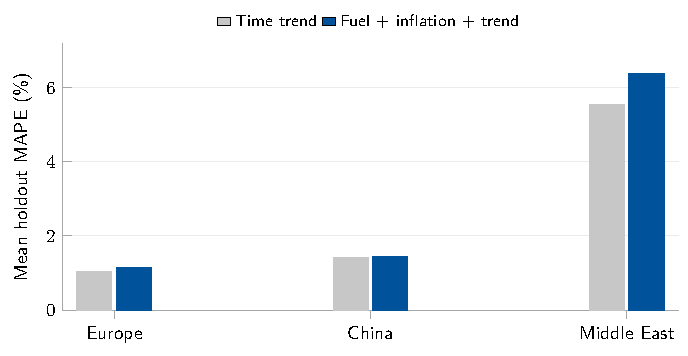
\includegraphics[width=\linewidth]{holdout_comparison.pdf}
\column{0.34\textwidth}
\lead{Improvement over a time trend}
\small Positive incremental out-of-sample $R^2$:\\[0.25cm]
\begin{tabular}{@{}lr@{}}
China & 8/27\\
Europe & 6/27\\
Middle East & 6/27
\end{tabular}
\par\vspace{0.25cm}
{\scriptsize\color{PaperGray}Training: 2026--2032.\\ Testing: 2033--2035.\par}
\end{columns}
\source{Ridge diagnostics on cleaned scenario panels; fixed holdout: 2033--2035. Counts compare fuel + inflation + trend against time trend alone.}
\end{frame}

\begin{frame}{Macroeconomic transmission}
\begin{tabularx}{\linewidth}{@{}Xllr@{}}
\toprule
\textbf{Target} & \textbf{Fuel} & \textbf{Lag} & \textbf{$p$-value}\\
\midrule
China real interest rate & Coal & 1 year & 0.00018\\[0.15cm]
China real interest rate & Coal & 2 years & 0.00691\\[0.15cm]
China real interest rate & Gas & 1 year & 0.01915\\[0.15cm]
Europe inflation & Gas & 2 years & 0.00952\\
\bottomrule
\end{tabularx}
\vspace{0.4cm}
\lead{Selected links appear through inflation and interest rates.}
\source{Selected Granger-style diagnostics on annual differenced targets and log-differenced fuel prices. Unadjusted exploratory $p$-values.}
\end{frame}

\begin{frame}{Regional policy implications}
\begin{tabularx}{\linewidth}{@{}p{0.18\linewidth}X X@{}}
\toprule
\textbf{Region} & \textbf{Relevant context} & \textbf{Financing question}\\
\midrule
Europe & Imported energy and policy credibility & How can predictable contracts and risk transfer support investment?\\[0.25cm]
China & International spillovers and domestic price regulation & How do public finance and price rules alter exposure?\\[0.25cm]
Middle East & Oil dependence and domestic energy-pricing institutions & How can financing capacity support diversification?\\
\bottomrule
\end{tabularx}
\source{Polzin et al. (2019); He and Lin (2017); Karanfil and Omgba (2023); Fattouh and El-Katiri (2013).}
\end{frame}

\begin{frame}{Selected references}
\footnotesize
\begin{enumerate}
\item N. Ameli et al., ``Higher cost of finance exacerbates a climate investment trap in developing economies,'' \textit{Nature Communications}, 12, 4046, 2021.\quad\href{https://doi.org/10.1038/s41467-021-24305-3}{doi:10.1038/s41467-021-24305-3}
\item M. Calcaterra et al., ``Reducing the cost of capital to finance the energy transition in developing countries,'' \textit{Nature Energy}, 9, 1241--1251, 2024.\quad\href{https://doi.org/10.1038/s41560-024-01606-7}{doi:10.1038/s41560-024-01606-7}
\item L. Paranhos, ``Predicting inflation with recurrent neural networks,'' \textit{International Journal of Forecasting}, online 2025.\quad\href{https://doi.org/10.1016/j.ijforecast.2024.07.010}{doi:10.1016/j.ijforecast.2024.07.010}
\item F. Polzin et al., ``How do policies mobilize private finance for renewable energy?'' \textit{Applied Energy}, 236, 1249--1268, 2019.\quad\href{https://doi.org/10.1016/j.apenergy.2018.11.098}{doi:10.1016/j.apenergy.2018.11.098}
\end{enumerate}

\end{frame}



\begin{frame}[t]{Conclusions}
\vspace{0.30cm}
\begin{columns}[T,onlytextwidth]
\column{0.53\textwidth}
\small
\begin{enumerate}
\item Fuel-price and inflation forecasts feed regional WACC scenarios.
\item Fit differs across regions and technologies.
\item Time-split checks show where price signals add information.
\end{enumerate}
\vspace{0.1cm}
{\small\textbf{\PresenterName}\\\PaperAffiliation\\
\href{mailto:shilin.ou@dukekunshan.edu.cn}{\PresenterEmail}\par}
\column{0.42\textwidth}
\vspace{0.15cm}
\begin{columns}[T,onlytextwidth]
\column{0.48\textwidth}\centering
\qrcode[height=2.25cm]{https://github.com/GreenComp-ERC/ImpactOfFossilFeulPrice}\\[0.25cm]
\scriptsize\textbf{Code + materials}
\column{0.48\textwidth}\centering
\qrcode[height=2.25cm]{https://huggingface.co/datasets/global-nomad-nexus/ImpactOfFossilFuelPrice-WACC}\\[0.25cm]
\scriptsize\textbf{Dataset snapshot}
\end{columns}
\vspace{0.45cm}
\smalllabel{Paper, code, data, and editable LaTeX sources.}
\end{columns}
\source{Corresponding authors: Luyao Zhang, \href{mailto:luyao.zhang@dukekunshan.edu.cn}{luyao.zhang@dukekunshan.edu.cn}; Ming-Chun Huang, \href{mailto:mingchun.huang@dukekunshan.edu.cn}{mingchun.huang@dukekunshan.edu.cn}.}
\note{\CorrespondenceText\par\FundingText\par\AuthorNoteText\par\PreparationText}
\end{frame}

\end{document}
